\documentclass[12pt, twoside]{article}
\usepackage[letterpaper, margin=1in, head=30pt, headsep=0.1in]{geometry}
\usepackage[english]{babel}
\usepackage[utf8]{inputenc}
\usepackage{amsmath}
\usepackage{amsfonts}
\usepackage{amssymb}
\usepackage{tikz}
\usetikzlibrary{quotes, angles}

\usepackage{graphicx}
\usepackage{enumitem}
\usepackage{multicol}

%\usepackage{pgfplots}
%\pgfplotsset{width=10cm,compat=1.9}
%\usepgfplotslibrary{statistics}
%\usepackage{pgfplotstable}
%\usepackage{tkz-fct}
%\usepackage{venndiagram}

\usepackage{fancyhdr}
\pagestyle{fancy}
\fancyhf{}
\renewcommand{\headrulewidth}{0pt} % disable the underline of the header
\raggedbottom
\newif\ifmeta
\metatrue %print standards and topics tags

\title{High School Geometry problem sets}
\author{Chris Huson}
\date{March 2021}

%\fancyhead[RE]{\thepage}
%\fancyhead[RO]{\thepage \\ Name: \hspace{3cm}}
%\fancyhead[L]{BECA / Dr. Huson / 10th Grade Geometry\\* 7 June 2019}
%
%\begin{document}
%\subsubsection*{13.7 Homework: Cross sections, distance applications}
%\fancyhead[L]{BECA / Dr. Huson / Geometry 03-Volume+angle-bisectors\\* pset ID: 34}

\begin{document}

\subsubsection*{7.7 Circle arc measures and lengths}
\begin{enumerate}
\item Do Now: What is the equation of a circle with center $(-2,5)$ and radius $r=4$?\\[0.5cm]
Graph the circle in Graspable Math or Geogebra and paste the image here.
%https://graspablemath.com/canvas?load=_6a89b545540e2be5

\newpage
\item Do Now: What are the coordinates of the center and the length of the radius of the circle whose equation is $(x-7)^2+(y+1)^2=9$?\\[0.5cm]
Graph the circle in Graspable Math or Geogebra and paste the image here.
%https://graspablemath.com/canvas?load=_6a89b545540e2be5

\newpage
\item Given circle $O$ with various internal line segments as shown.
    \begin{multicols}{2}
    \raggedcolumns
    \begin{enumerate}[itemsep=0.5cm]
      \item Highlight each radius in red
      \item Highlight any chords in yellow
      \item Is the $\angle CAD$ an inscribed angle or a central angle?
      \item Is $\triangle AOB$ an equilateral triangle, isosceles triangle, or a scalene triangle?
      
    \end{enumerate}
    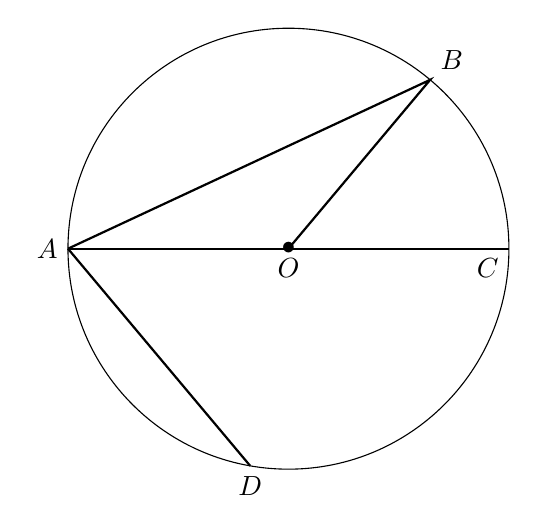
\begin{tikzpicture}[scale=0.7]
      \draw (0,0) circle[radius=4];
      \draw [thick]
      (-4,0) node[left] {$A$}--
      (0,0) node[below] {$O$}--
      (4,0) node[below left] {$C$};
      \draw [thick]
      (0,0) -- (50:4) node[above right] {$B$}--(-4,0);
      \draw [thick]
      (-4, 0)--
      (-100:4) node[below] {$D$};
      \node at (0,0) {$\bullet$};
    \end{tikzpicture}
    \end{multicols}

\newpage
\item Given circle $O$ with points on the circle $A$, $B$, $C$, $D$ as shown. Find each central angle measure.
  \begin{multicols}{2}
    \begin{enumerate} 
      \item $m\angle AOB =$
      \item $m\angle BOC =$
      \item $m\angle AOC =$
      \item What is the measure of the \emph{reflex angle} $m\angle AOC =$, i.e. the one containing point $D$ that is $>180^\circ$
      \end{enumerate}
      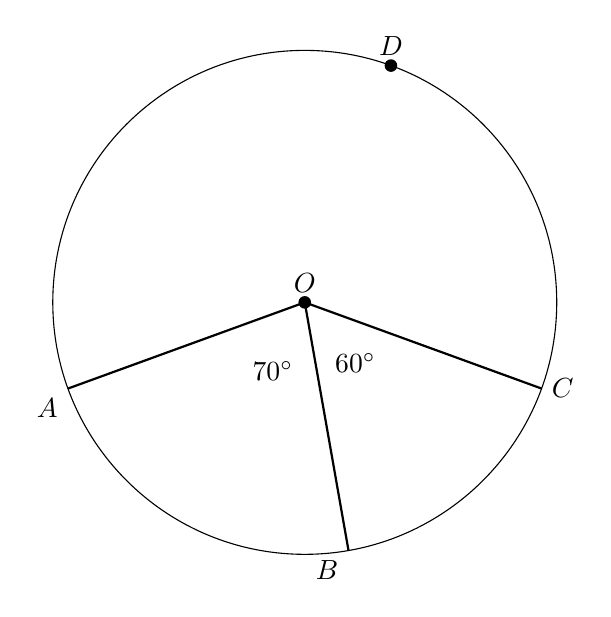
\begin{tikzpicture}[scale=0.8]
        \draw (0,0) circle[radius=4];
        \draw [thick]
        (-80:4) node[below left] {$B$}--
        (0,0) node[above] {$O$}--
        (-160:4) node[below left] {$A$};
        \draw [thick]
        (0,0) -- (-20:4) node[right] {$C$};
        %\node at (0,0) {$\bullet$};
        \fill (0,0) circle[radius=.1];
        \fill (70:4) circle[radius=.1]node[above]{$D$};
        \node at (-50:1.25) {$60^\circ$};
        \node at (-115:1.2) {$70^\circ$};
      \end{tikzpicture}
  \end{multicols}

\newpage
\item Lesson: Given circle $O$ with points on the circle $A$, $B$, $C$, $D$, $E$.
    \begin{multicols}{2}
    \raggedcolumns
    \begin{enumerate}[itemsep=0.5cm]
      \item Highlight the two radii $\overline{OD}$ and $\overline{OE}$
      \item The segments $\overline{AB}$ and $\overline{AC}$ are called \emph{chords} (pronounced with a hard ``c'', \emph{kord})
      \item The angle with the circle's center as its vertex is called a \emph{central angle}, $\angle DOE$
      \item The angle with its vertex on the circle is called an \emph{inscribed angle}, $\angle BAC$
    \end{enumerate}
    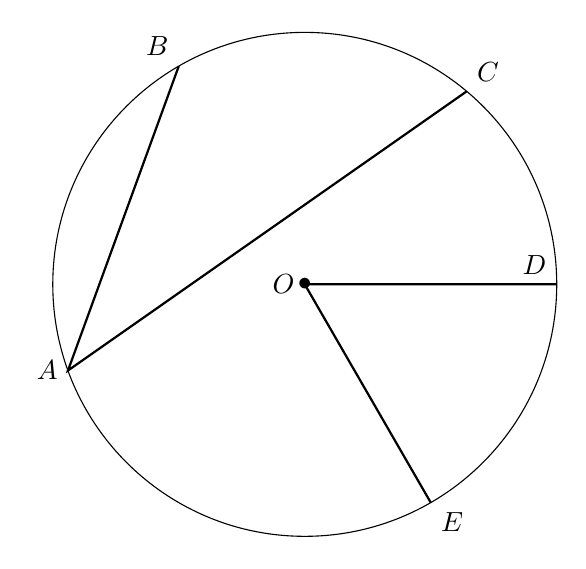
\begin{tikzpicture}[scale=0.8]
      \draw (0,0) circle[radius=4];
      \draw [thick]
      (0:4) node[above left] {$D$}--
      (0,0) node[left] {$O$}--
      (-60:4) node[below right] {$E$};
      \draw [thick]
      (120:4) node[above left] {$B$}--
      (200:4) node[left] {$A$}--
      (50:4) node[above right] {$C$};
      \node at (0,0) {$\bullet$};
    \end{tikzpicture}
    \end{multicols}
    
\newpage
\item What is an equation of circle O shown in the graph below?
  \begin{center}
    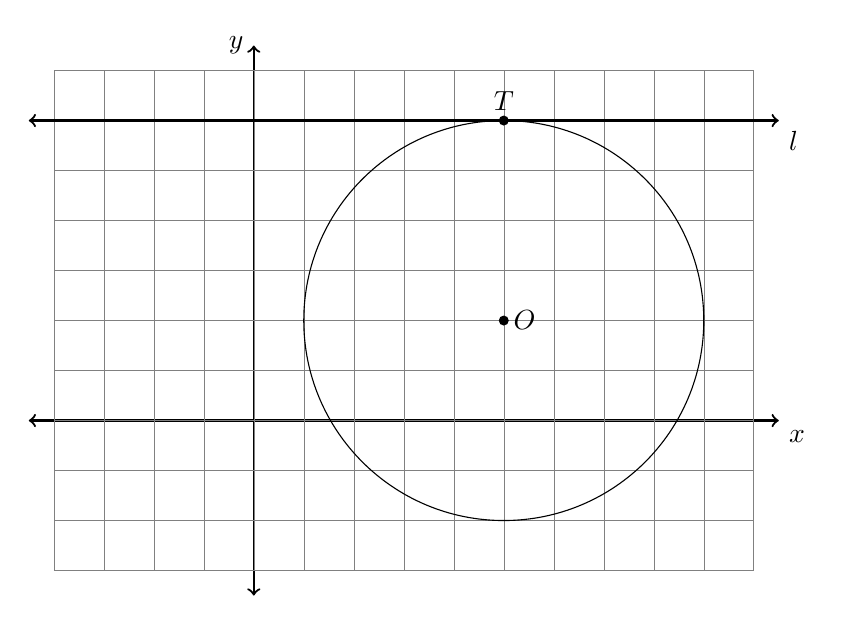
\begin{tikzpicture}[scale=.635]
      \draw [thick, <->] (-4.5,0) -- (10.5,0) node [below right] {$x$};
      \draw [thick, <->] (0,-3.5)--(0,7.5) node [left] {$y$};
      \draw [help lines] (-4,-3) grid (10,7);
      \draw (5,2) circle[radius=4];
      \fill (5,2) circle[radius=.1]node[right]{$O$};
      \draw [thick, <->] (-4.5,6) -- (10.5,6) node [below right] {$l$};
      \fill (5,6) circle[radius=.1]node[above]{$T$};
    \end{tikzpicture}
  \end{center}
  \begin{multicols}{2}
    \begin{enumerate}
      \item $(x-5)^2+(y-2)^2=16$
      \item $(x+5)^2+(y+2)^2=8$
      \item $(x+2)^2+(y+5)^2=8$
      \item $(x-2)^2+(y-5)^2=16$
    \end{enumerate}
  \end{multicols}
  Write down the coordinates of the point of tangency $T$ and the equation of the tangent line $l$.

\newpage
\item Given circle $O$ with points on the circle $A$, $B$, $C$, $D$ as shown. Find each central angle measure.
\begin{multicols}{2}
  \begin{enumerate} 
    \item $m\angle AOB =$
    \item $m\angle BOC =$
    \item $m\angle AOC =$
    \item What is the measure of the \emph{reflex angle} $m\angle AOC =$, i.e. the one containing point $D$ that is $>180^\circ$
    \end{enumerate}
\columnbreak
    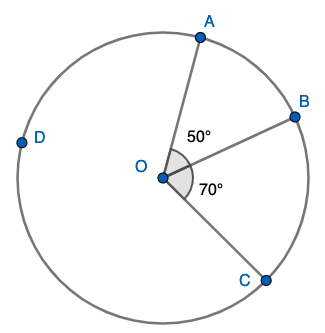
\includegraphics[width=7.5cm]{7-6-7_central_angles.png}
    https://www.geogebra.org/calculator/xqketuwj
\end{multicols}
     
\newpage
\item What are the coordinates of the center and the length of the radius of the circle whose equation is $(x+4)^2+(y-3)^2=16$?
    \begin{enumerate}
      \item center $(-4,3)$ and radius 8
      \item center $(4,-3)$ and radius 4
      \item center $(-4,3)$ and radius 4
      \item center $(4,-3)$ and radius 8
    \end{enumerate}

\newpage
\item What is the equation of a circle with center $(-3,7)$ and radius $r=6$?\\[0.5cm]
  Graph the circle in Graspable Math or Geogebra and paste the image here.
  %https://graspablemath.com/canvas?load=_6a89b545540e2be5

\newpage
\item Given $A(-1,2)$ and $B(3,5)$, find the length of $\overline{AB}$. Show the substitution into the distance formula.
\item %https://graspablemath.com/canvas?load=_024bda2a5587c074
      
\newpage
\item Find the volume of a pyramid ($V=\frac{1}{3}Bh$) having a height of 11.3 inches and with a square base having side lengths of 7 inches. Express your result to the \emph{nearest cubic inch}. \vspace{5cm}

\newpage
\item Find the volume of a hemisphere with a radius of 30 inches, to the \emph{nearest whole cubic inch}. (The formula for the volume of a \emph{sphere} is $V=\frac{4}{3}\pi r^3$ and a \emph{hemisphere} is half of a sphere.) \vspace{5cm}

\end{enumerate}
\end{document}